%%%%%%%%%%%%%%%%%%%%%%%%%%%%%%%%%%%%%%
% Multiplicative domain poster
% Created by Nathaniel Johnston
% August 2009
% http://www.nathanieljohnston.com/2009/08/latex-poster-template/
%%%%%%%%%%%%%%%%%%%%%%%%%%%%%%%%%%%%%%

\documentclass[final]{beamer}
\usepackage[scale=1.24]{beamerposter}
\usepackage{graphicx}			% allows us to import images

%-----------------------------------------------------------
% Custom commands that I use frequently
%-----------------------------------------------------------

\newcommand{\bb}[1]{\mathbb{#1}}
\newcommand{\cl}[1]{\mathcal{#1}}
\newcommand{\fA}{\mathfrak{A}}
\newcommand{\fB}{\mathfrak{B}}
\newcommand{\Tr}{{\rm Tr}}
\newtheorem{thm}{Theorem}

%-----------------------------------------------------------
% Define the column width and poster size
% To set effective sepwid, onecolwid and twocolwid values, first choose how many columns you want and how much separation you want between columns
% The separation I chose is 0.024 and I want 4 columns
% Then set onecolwid to be (1-(4+1)*0.024)/4 = 0.22
% Set twocolwid to be 2*onecolwid + sepwid = 0.464
%-----------------------------------------------------------

\newlength{\sepwid}
\newlength{\onecolwid}
\newlength{\twocolwid}
\setlength{\paperwidth}{1189mm}
\setlength{\paperheight}{841mm}
\setlength{\sepwid}{0.024\paperwidth}
\setlength{\onecolwid}{0.22\paperwidth}
\setlength{\twocolwid}{0.464\paperwidth}
\setlength{\topmargin}{-0.5in}
\usetheme{confposter}
\usepackage{exscale}
\usepackage{graphicx}
%\usepackage{subcaption}
\usepackage{array}
\usepackage{booktabs}% http://ctan.org/pkg/booktabs
\usepackage{multicol}

\newcommand{\tabitem}{~~\llap{\textbullet}~~}
\def\LW{\dimexpr.2\linewidth-.0em}


%-----------------------------------------------------------
% The next part fixes a problem with figure numbering. Thanks Nishan!
% When including a figure in your poster, be sure that the commands are typed in the following order:
% \begin{figure}
% \includegraphics[...]{...}
% \caption{...}
% \end{figure}
% That is, put the \caption after the \includegraphics
%-----------------------------------------------------------

\usecaptiontemplate{
\small
\structure{\insertcaptionname~\insertcaptionnumber:}
\insertcaption}

%-----------------------------------------------------------
% Define colours (see beamerthemeconfposter.sty to change these colour definitions)
%-----------------------------------------------------------

\setbeamercolor{block title}{fg=ngreen,bg=white}
\setbeamercolor{block body}{fg=black,bg=white}
\setbeamercolor{block alerted title}{fg=white,bg=dblue!70}
%\setbeamercolor{block alerted body}{fg=black,bg=dblue!10}
\setbeamercolor{block alerted body}{fg=black,bg=white}


%-----------------------------------------------------------
% Name and authors of poster/paper/research
%-----------------------------------------------------------

%\title{\parbox[c]{38in}{Lineage diversification in the genus \textit{Solanum }L. (Solanaceae)}
%\parbox[c]{5in{\includegraphics[width=5in]{./logos/ICL_logo.PNG}}\\ \includegraphics[width=5in]{./logos/ICL_logo.PNG}}}
\title{Plant functional diversity and the biogeography of biomes in North and South America}
\author{Susy Echeverr\'ia-Londo\~no$^{1*}$, Brian J. Enquist$^{2}$, Danilo M. Neves$^{2}$, Cyrille Violle$^{3}$ \& Andrew J, Kerkhoff$^{1}$}
\institute{\small (1) Department of Biology, Kenyon College, Gambier, Ohio, USA; (2) Department of Ecology and Evolutionary Biology, University of Arizona, Tucson, Arizona, USA; (3) Centre d'Ecologie Fonctionnelle et Evolutive (UMR 5175), CNRS, Universit\'e de Montpellier, Universit\'e Paul Val\'ery, Montpellier, France \\ *echeverrialondono1@kenyon.edu}

%-----------------------------------------------------------
% Start the poster itself
%-----------------------------------------------------------
% The \rmfamily command is used frequently throughout the poster to force a serif font to be used for the body text
% Serif font is better for small text, sans-serif font is better for headers (for readability reasons)
%-----------------------------------------------------------

\begin{document}
 \small
\begin{frame}[t]
  \begin{columns}[t]												% the [t] option aligns the column's content at the top
    \begin{column}{\sepwid}\end{column}			% empty spacer column
    \begin{column}{\onecolwid}

     
      \begin{block}{Introduction}

Understanding functional differences among biomes is critically important to modeling the global carbon cycle and the functioning of the Earth system, including responses to anthropogenic global change. Our goals in this study are (1) to document the extent of the available data that characterize the functional diversity and distinctiveness of biomes, to highlight persistent data shortfalls. (2) Given the available data, we quantify the functional distinctiveness of a biome by identifying the most common functional strategies of the most widespread species within it. (3) we explore whether biomes are in fact characterized by functionally distinct collections of species using measures of functional similarity based on multidimensional hypervolumes in functional trait space. 

      \end{block}
      \vskip2ex
      

     \begin{block}{Methods}
     
     

We used the BIEN database to extract range maps and trait measurements of plant species distributed in North and South America. The BIEN (Botanical Information and Ecology Network) database integrates standardized plant observations stemming from herbarium specimens and vegetation plot inventories (Enquist, B.J. et al. 2016, Goldsmith et al., 2016).

%\begin{figure}[h]
%	\centering
%	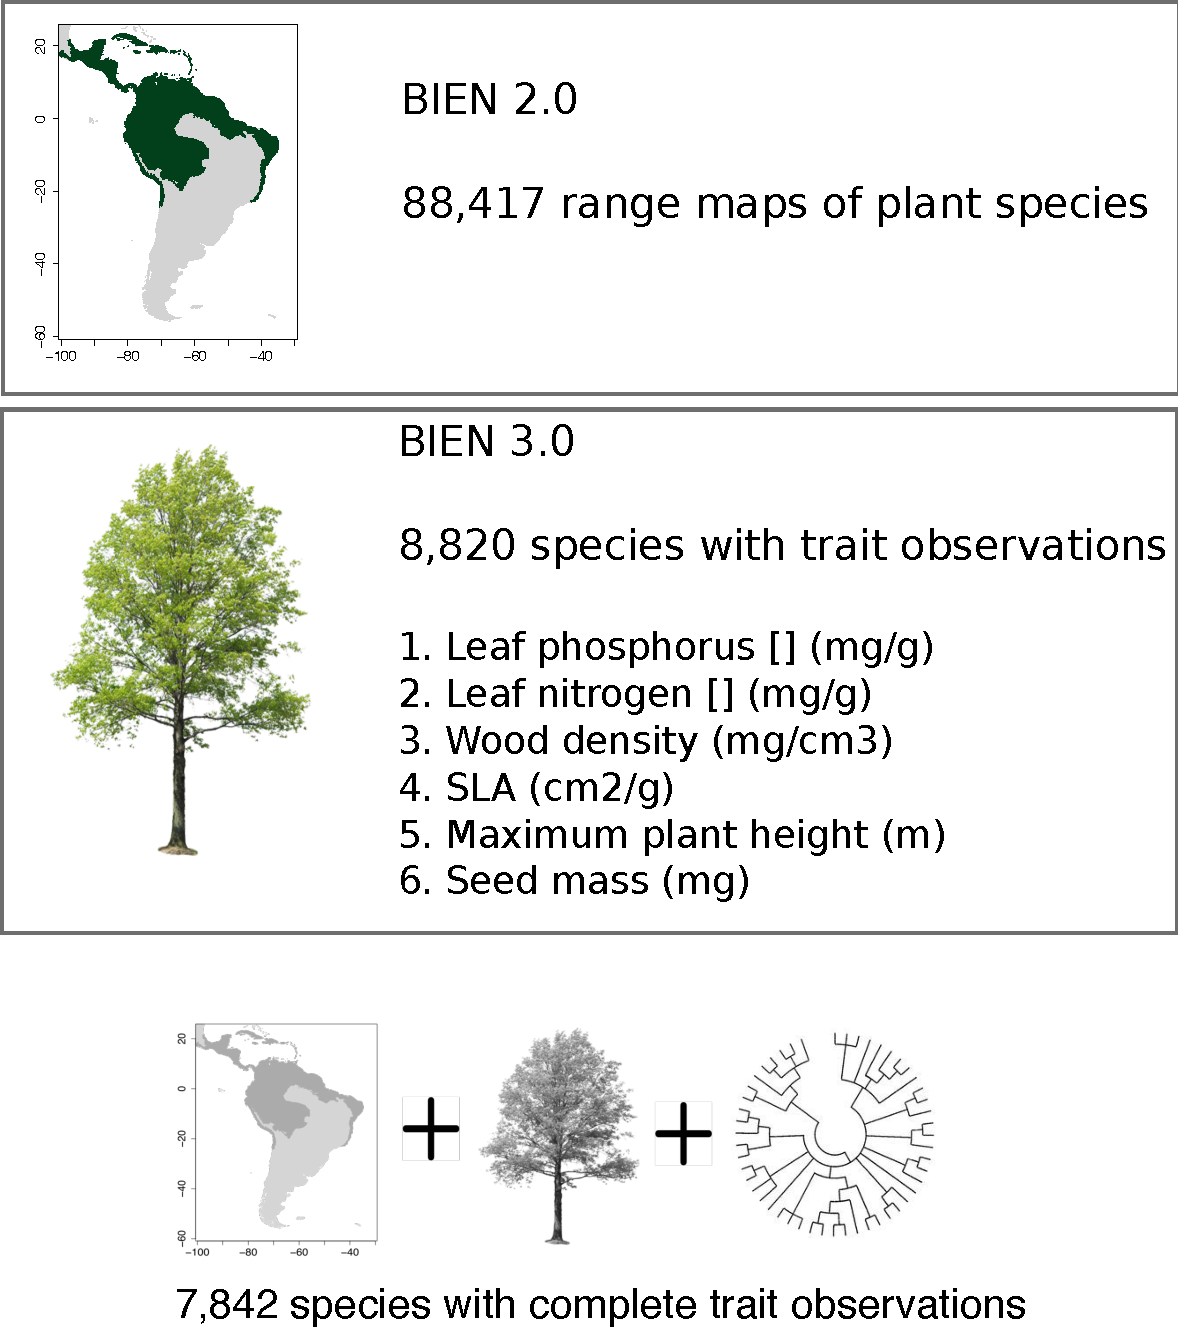
\includegraphics[width=0.5\textwidth]{./figures/Methods_figs.pdf}
%	%\includegraphics[scale=2]{./figures/Diversification_shifts_rate2.pdf}
%	\caption{}
%	\label{fig:methods}
%\end{figure}

\hfill

\begin{tabular}{cp{0.3\textwidth}cp{0.4\textwidth}}

	\begin{minipage}{.15\textwidth}
		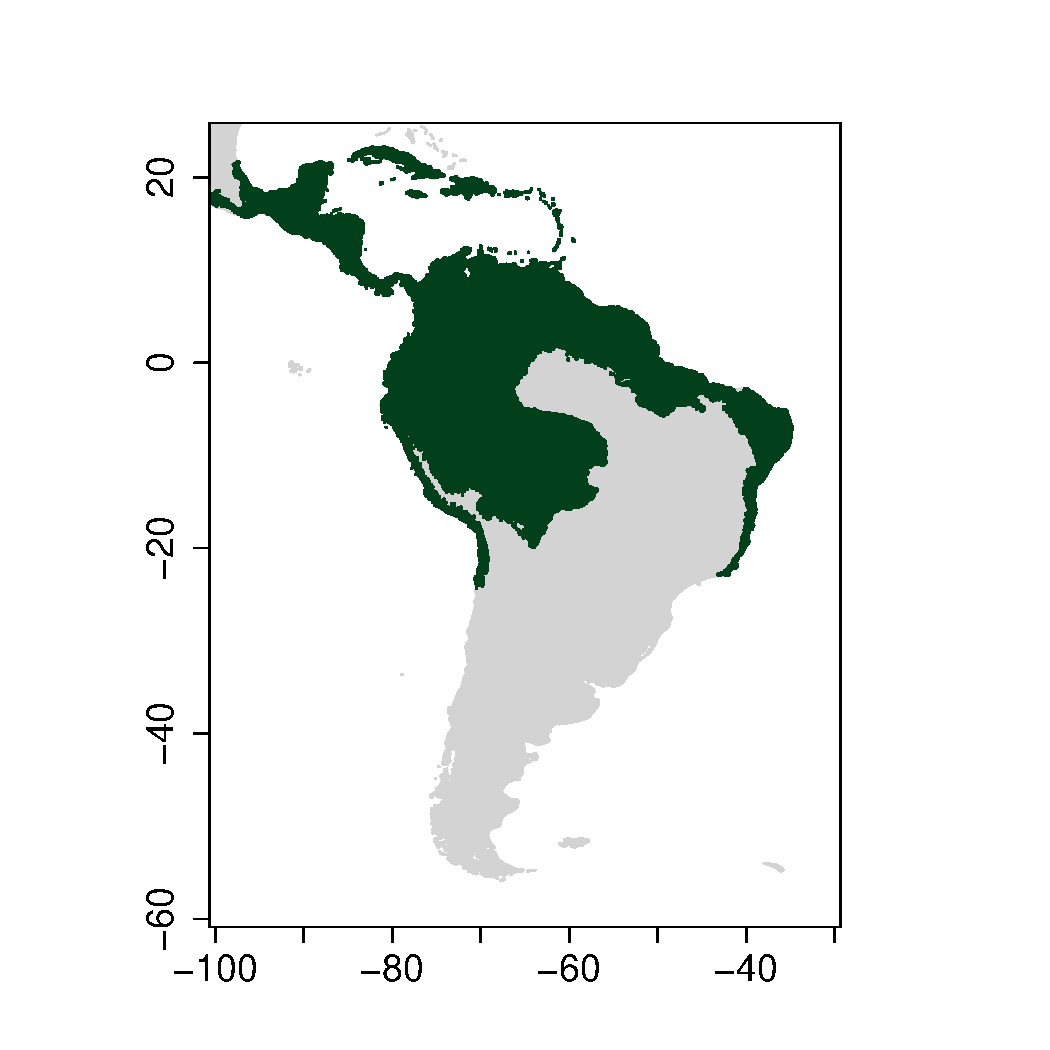
\includegraphics[width=\linewidth]{./figures/Range_maps_fig/Range_map_figure.pdf}
	\end{minipage} & 

\begin{itemize}
		\item BIEN 2.0 (range maps)
		\item 88,417 species
	\end{itemize} &

\begin{minipage}{.15\textwidth}
	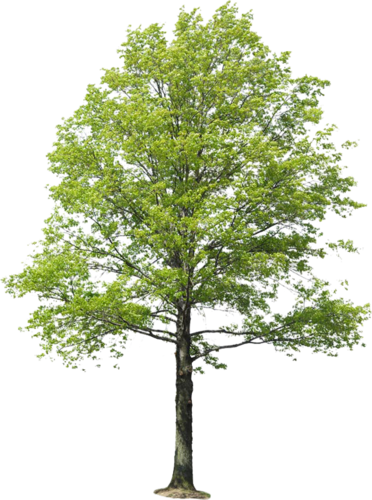
\includegraphics[width=\linewidth]{./figures/tree_fig.png}
\end{minipage} &

\begin{itemize}
	\item BIEN 3.0 (trait observations)
	\item 8,820 species
\end{itemize} \\ 


\multicolumn{4}{c}{} \\

\multicolumn{4}{c}{} \\


\multicolumn{4}{c}{ \hspace{0.25\textwidth} \begin{minipage}{\textwidth}
		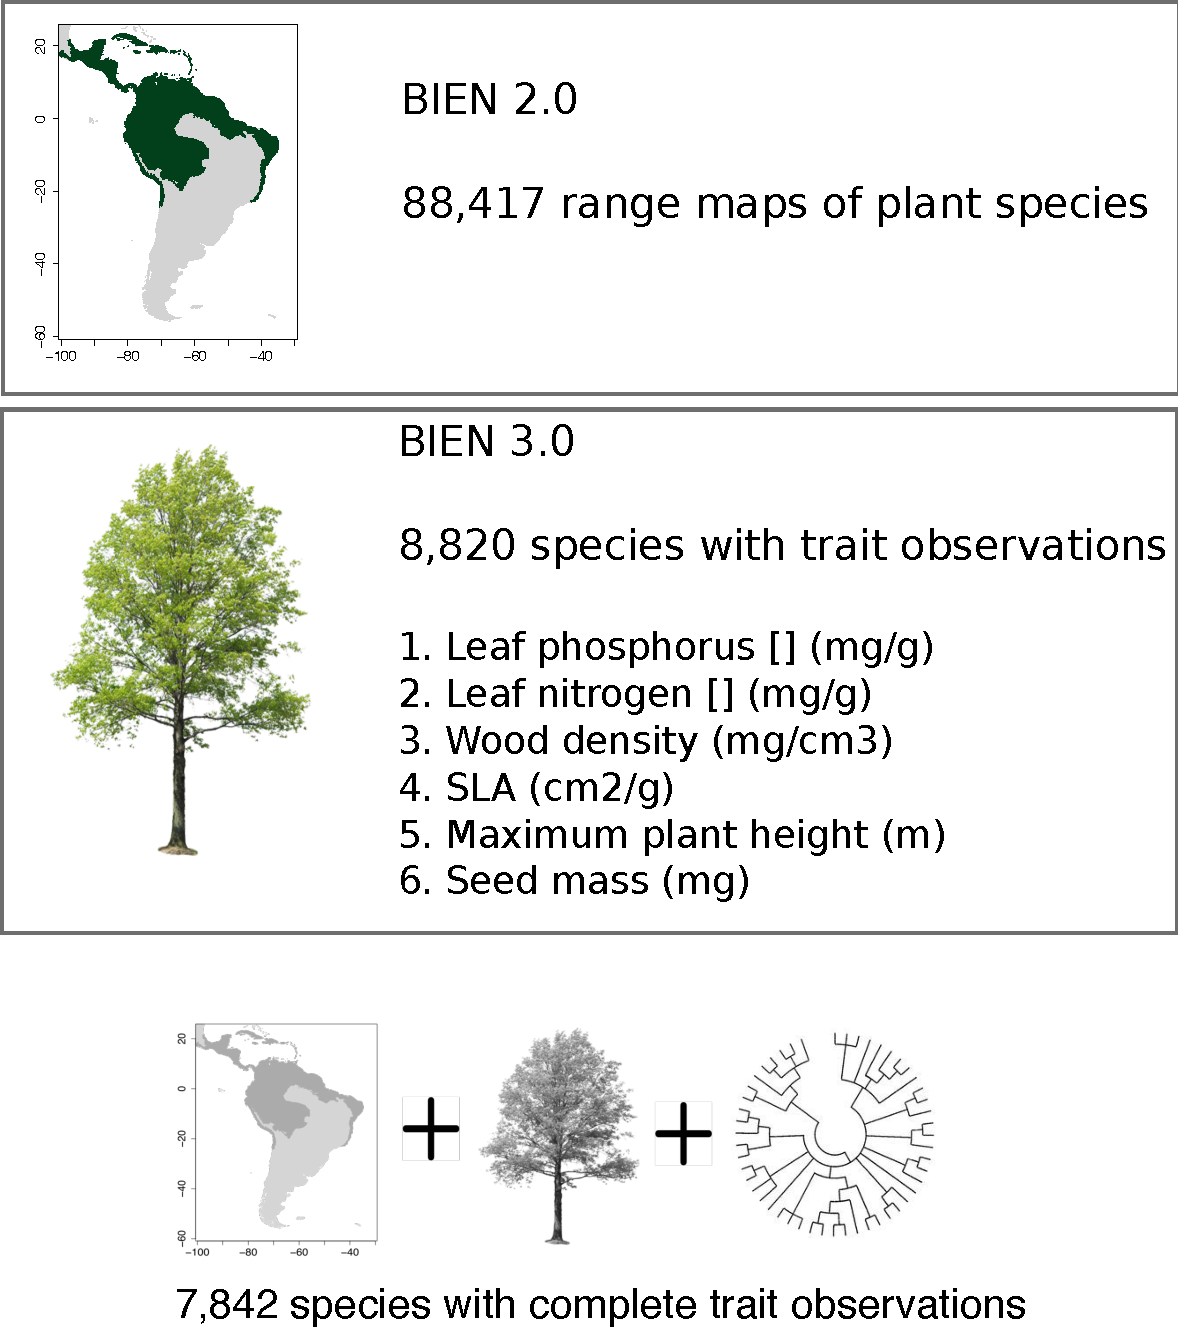
\includegraphics[width=0.5\linewidth]{./figures/Methods_figs.pdf} 
\end{minipage} } \\
\\ 
\multicolumn{4}{l}{ \hspace{0.09\textwidth} \textbf{7,842 species with complete trait information and range maps}}

\end{tabular}

\hfill

 To estimate the functional trait space for each biome, we require complete trait data. For this reason, we phylogenetically imputed missing trait data using the R package ``Rphylopars'' v 0.2.9 (Goolsby et al., 2017) and the recently published phylogeny of seed plants by (Smith and Brown, 2018) as a baseline (see Fig. \ref{fig:sampling}).

\begin{figure}[h]
	\centering
	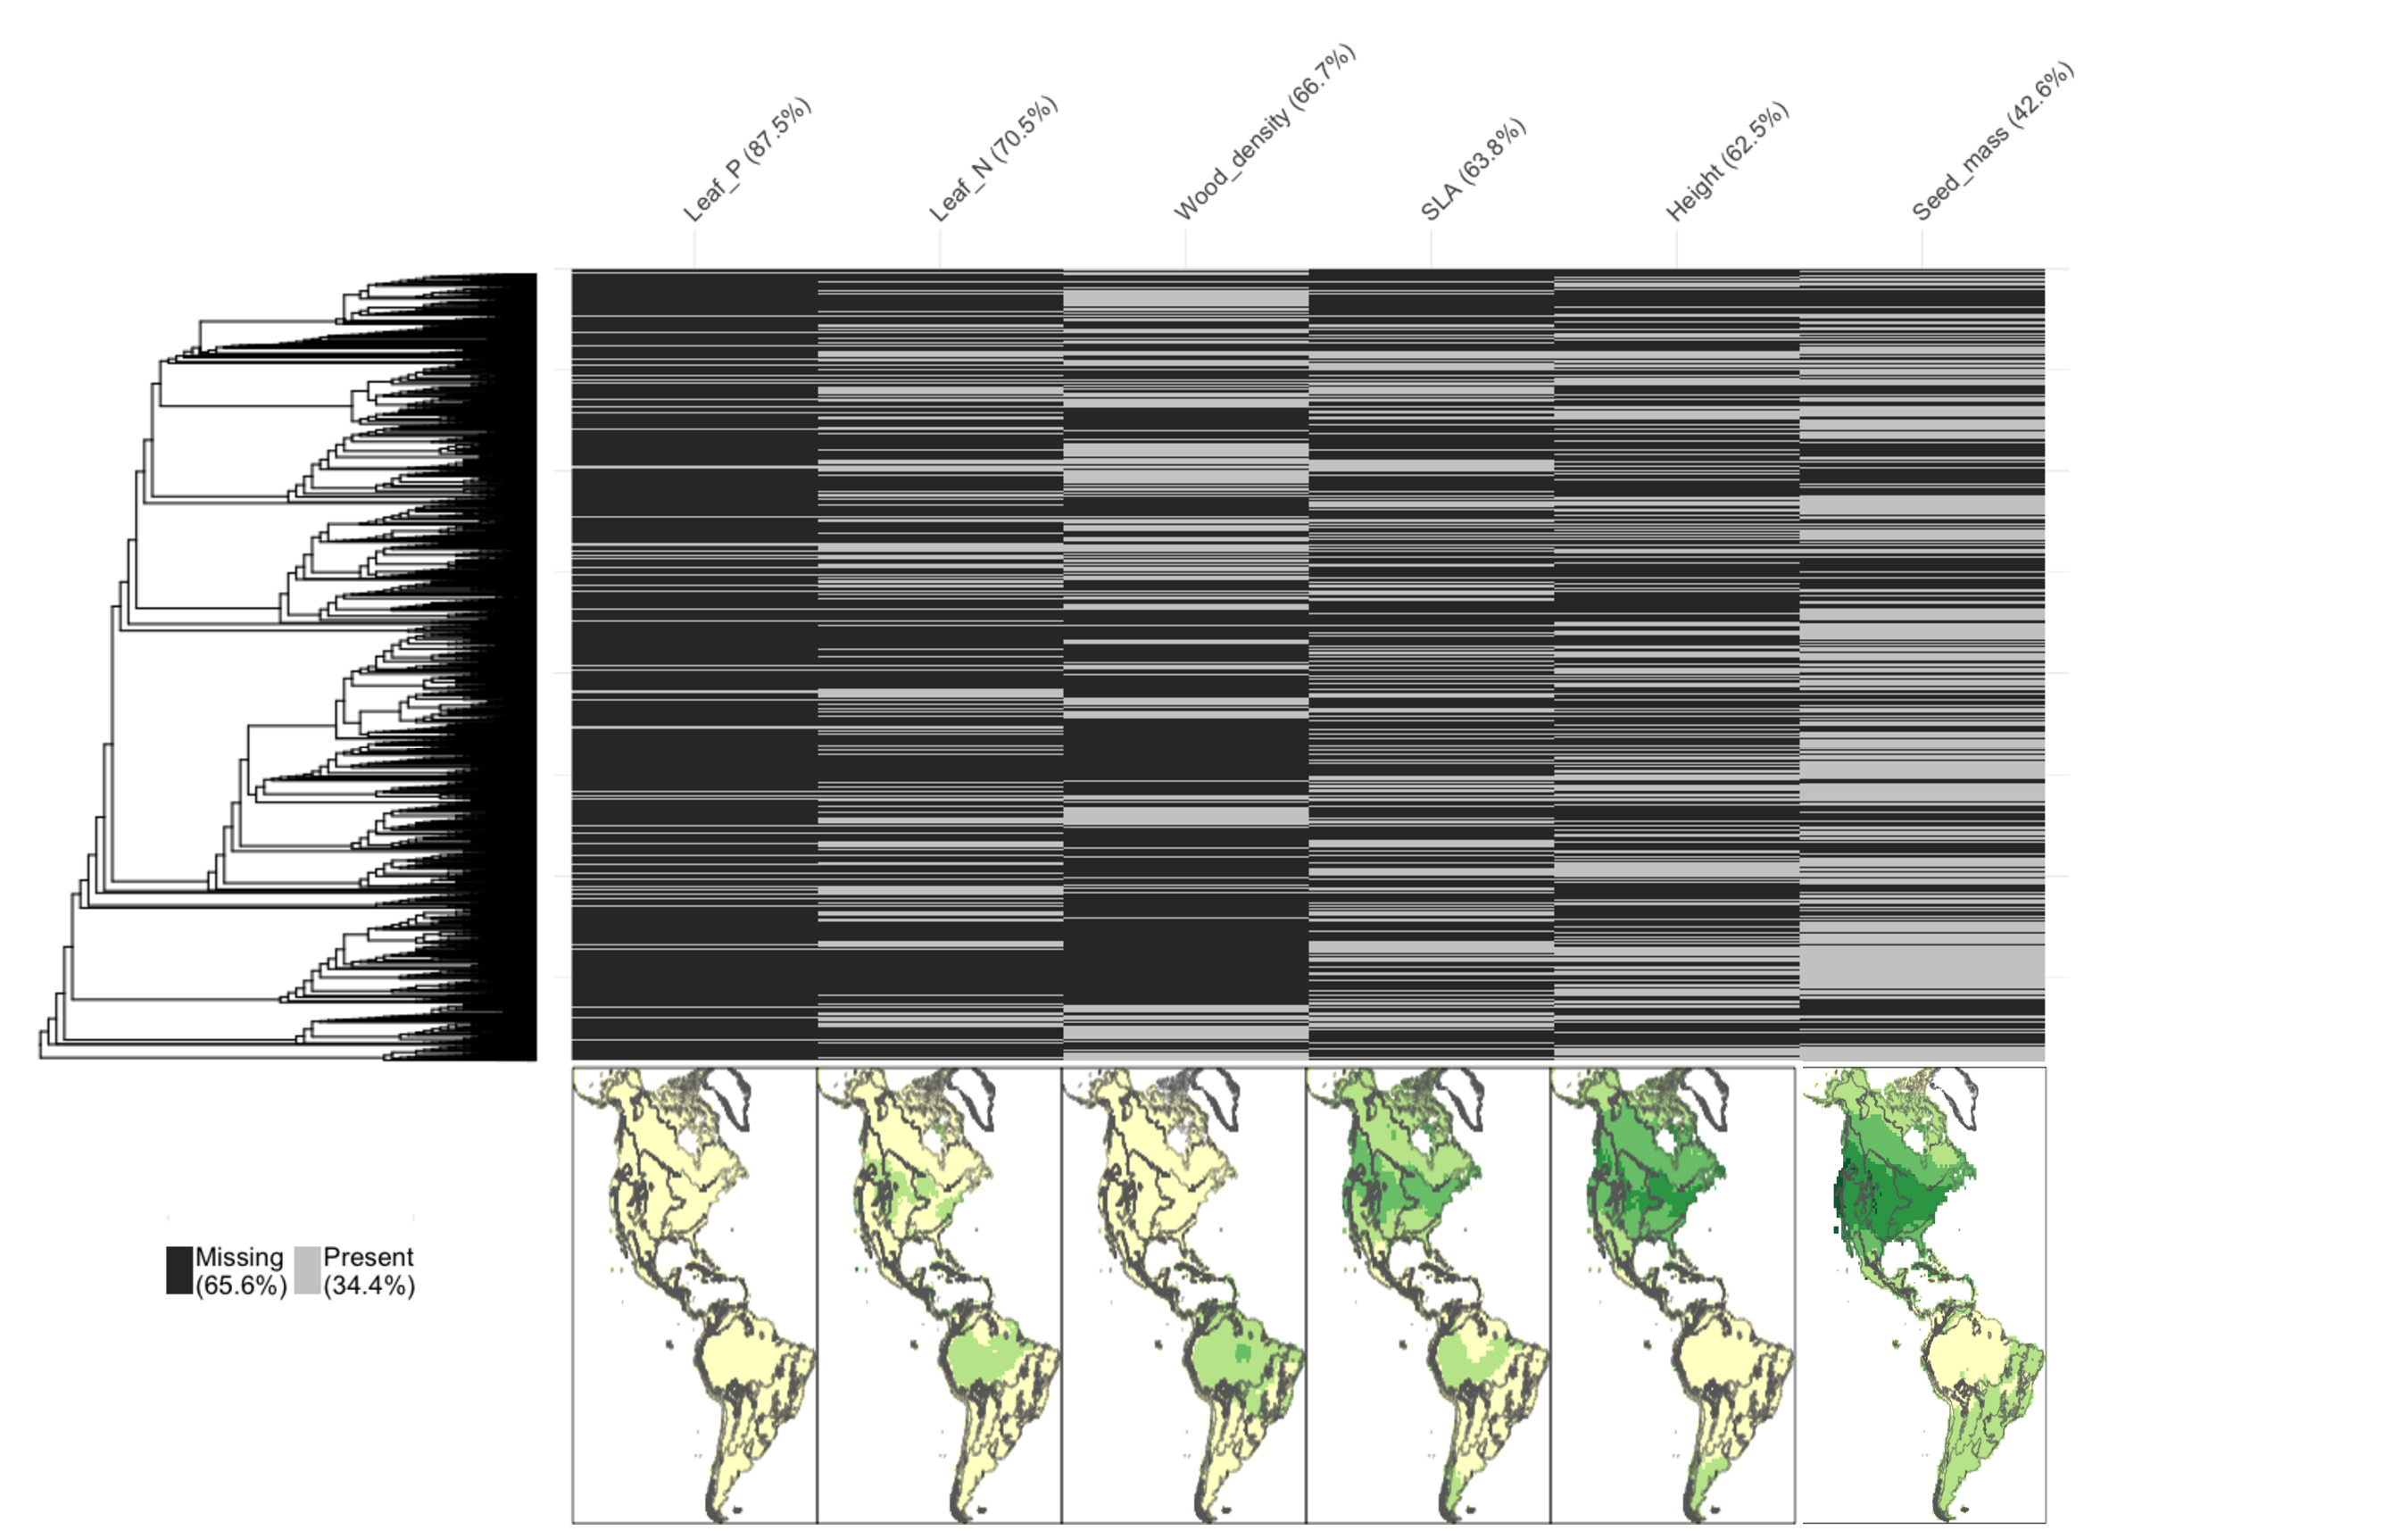
\includegraphics[width=1.05\textwidth]{./figures/Trait_sampling}
	\caption{Proportion of species with known (gray) or missing (black) trait values to the total number of species in the BIEN 3.0 database. Phylogeny at the left corresponds to the ALLBM tree from Smith and Brown, 2018}
	\label{fig:sampling}
\end{figure}

We measured the relative functional diversity of biomes by calculating trait hypervolumes from species pools within biomes cells. The hypervolumes for each grid cell, and collections of cells per biome,  were estimated using the extracted six functional traits and the R package ``hypervolume'' (Blonder et al., 2014, 2018), using the Gaussian KDE method with the default Silverman bandwidth estimator (see Fig. \ref{fig:map}B). Given the considerable overlap of species composition among biomes (see Fig. \ref{fig:map}A), we explore how widely species are distributed within biomes, and whether a species is more or less functionally similar to the rest of the community. Using the species geographical distribution and functional trait information, we estimate the functional distinctiveness and widespreadness of each species in each biome, following the conceptual framework of functional rarity by (Violle et al. 2017).

	\end{block}

    \end{column}


    \begin{column}{\sepwid}\end{column}			% empty spacer column
    \begin{column}{\twocolwid}							% create a two-column-wide column and then we will split it up later

\begin{figure}[h]
	\centering
	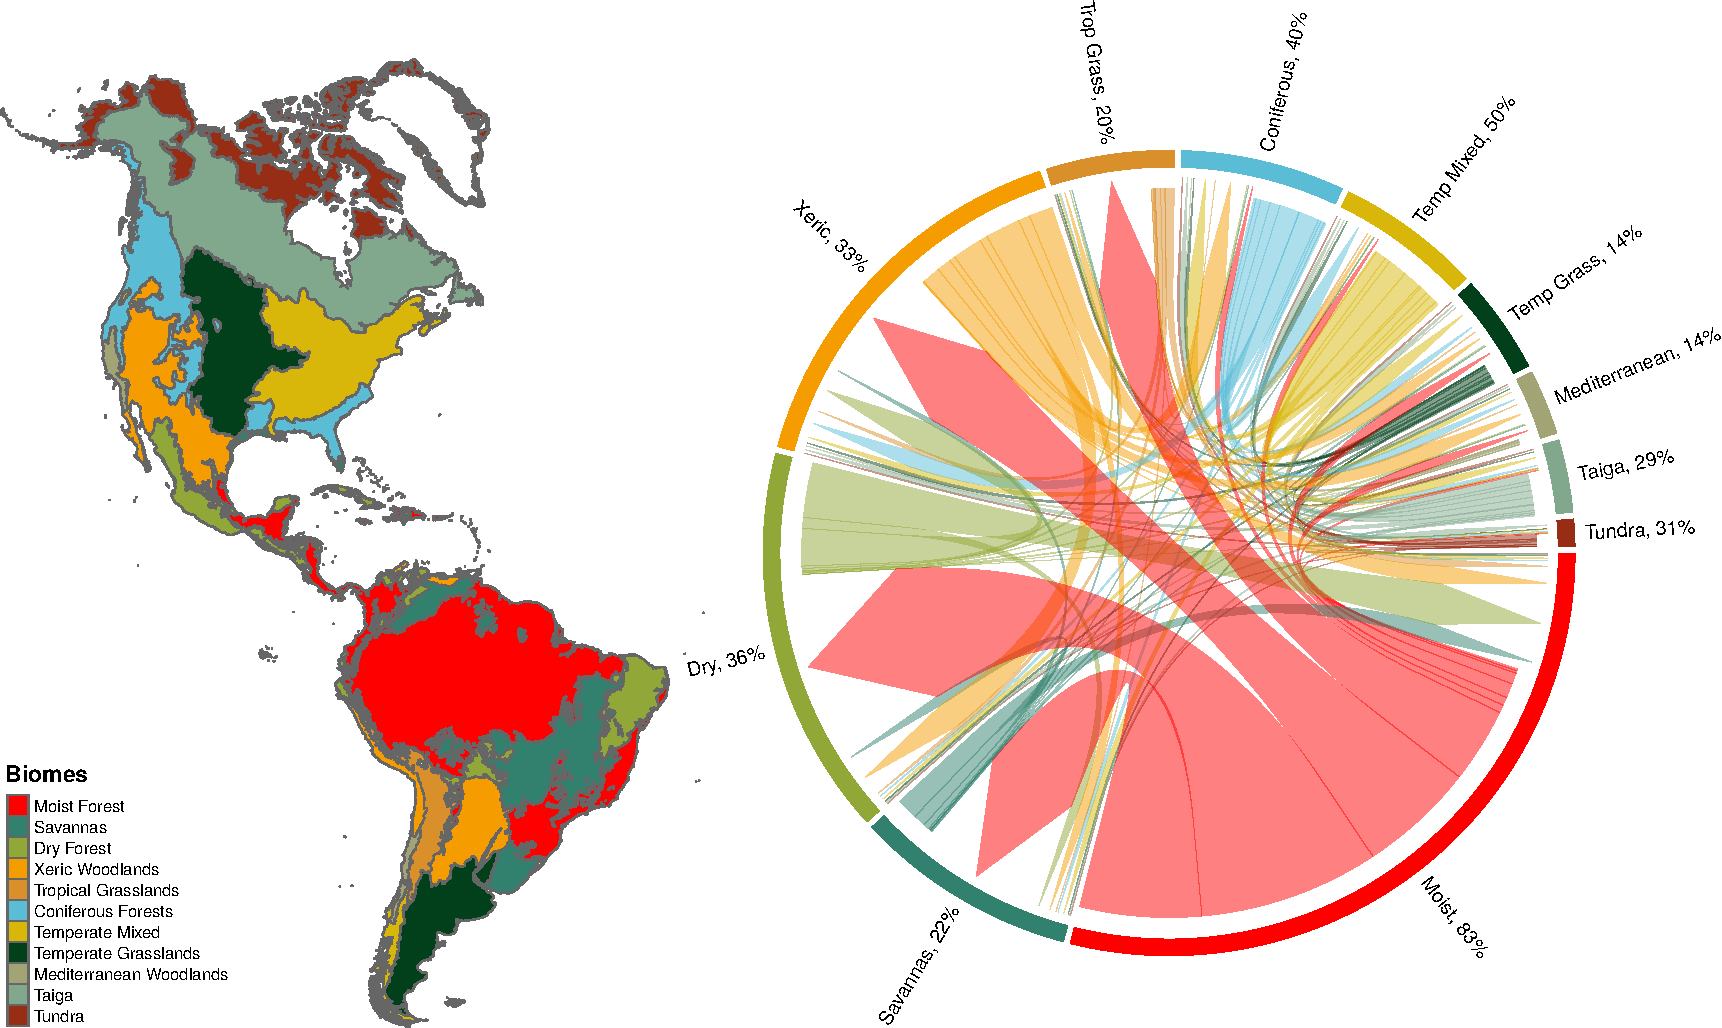
\includegraphics[width=0.75\textwidth]{./figures/Figure1.pdf}
	~
	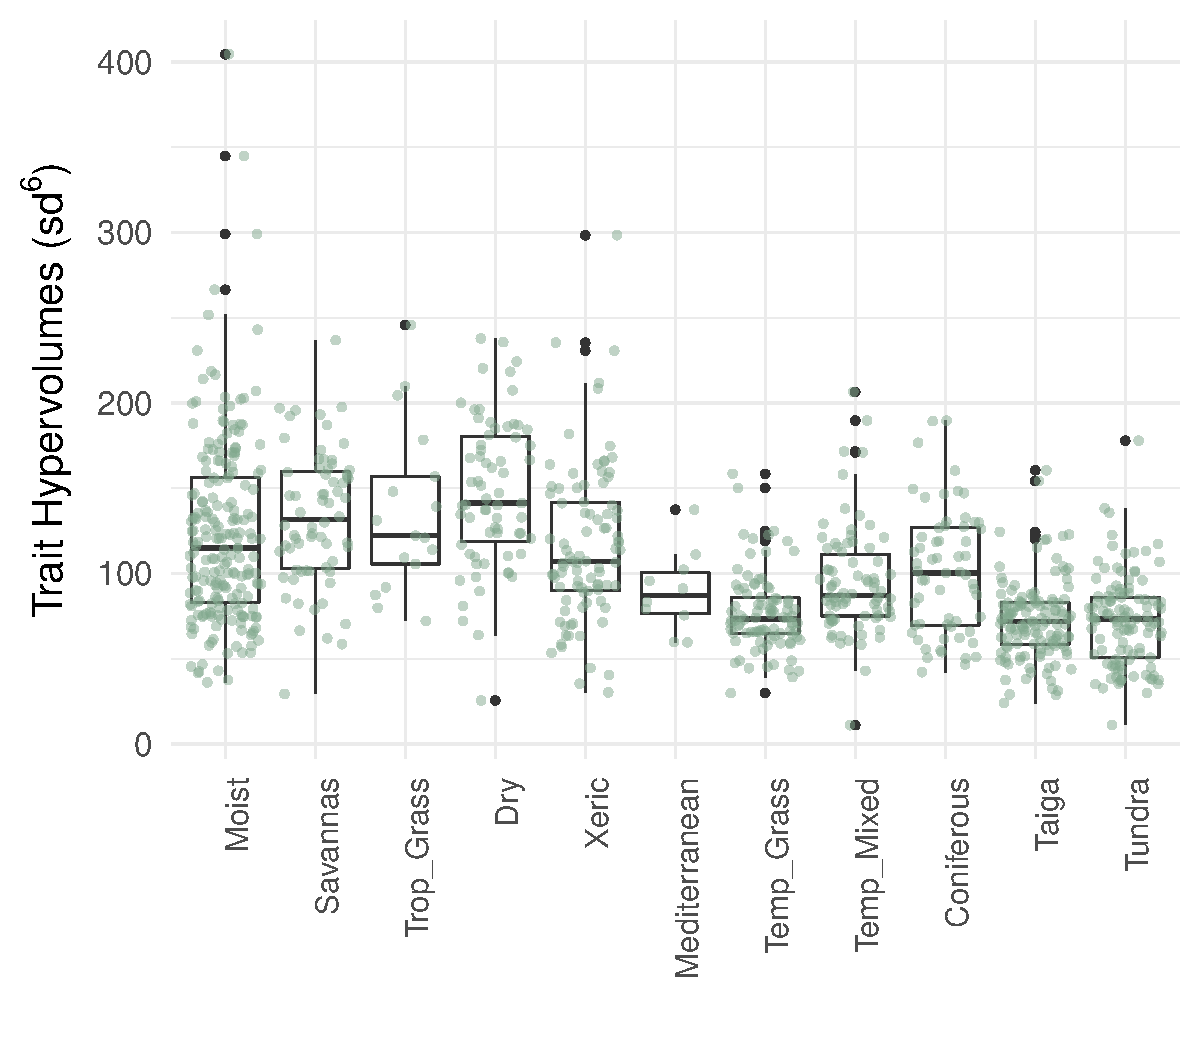
\includegraphics[width=0.25\textwidth]{./figures/Hypervolume_sp_sample_gaussian20perc.pdf}
	\caption{(A) Overlap of plant species among biomes of the New World. Percentage values express the fraction of species that have the greatest proportion of their geographic range in each biome. (B) Distribution of trait hypervolumes of 20\% of randomly selected 100X100 km cells in each biome. Hypervolumes are reported in units of standard deviations to the power of the number of traits used.}
	\label{fig:map}
\end{figure}



\begin{block}{Results}


		 
\begin{multicols}{2}

\begin{figure}[h]
	\centering
	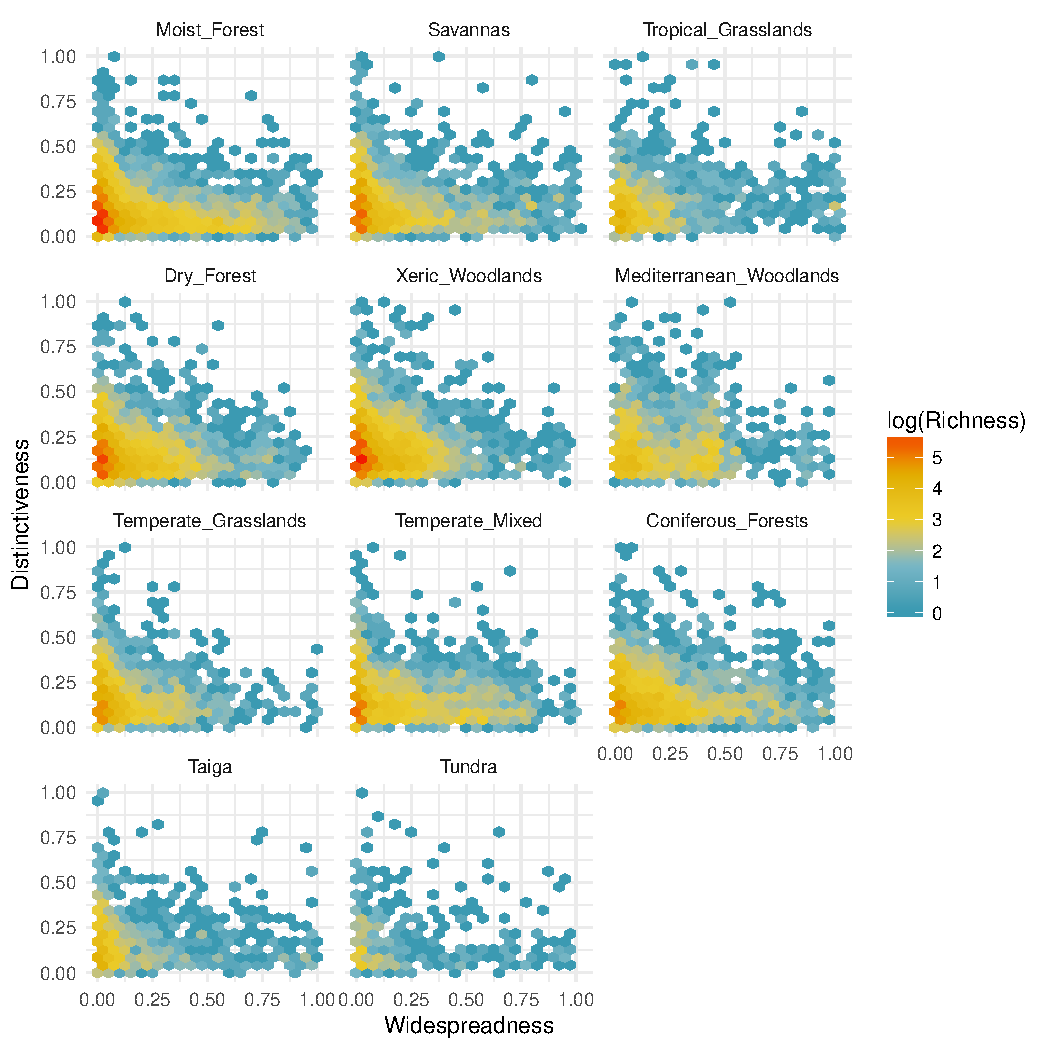
\includegraphics[width=0.39\textwidth]{./figures/All_biomes_heatmap_logTraits.pdf}
	\caption{Patterns of functional distinctiveness among biomes. Distinctiveness represents how species are functionally distant from another within a biome (i.e., the mean pairwise phenotypic distance from a focal species to all the others). The larger the value, the more distant a species is to the centroid of the biome's functional space. Widespreadness measures how geographically common a species is. A value of 0 indicates that a species is present in a single biome cell. }
	\label{fig:distinct_common}
\end{figure}


   Despite substantial hypervolume overlap among all the biomes (Fig \ref{fig:map}B), tropical, temperate, and cold biomes all appear to occupy distinguishable regions of functional space (Fig. \ref{fig:hypervolumes}). The main traits differentiating biomes appear to be traits related to overall plant size, including both mature height and seed mass (Fig. \ref{fig:hypervolumes}), rather than by leaf economics trait, as observed in more local, plot-based analyses (Douma et al., 2012).   		

\begin{figure}[h]
	\centering
	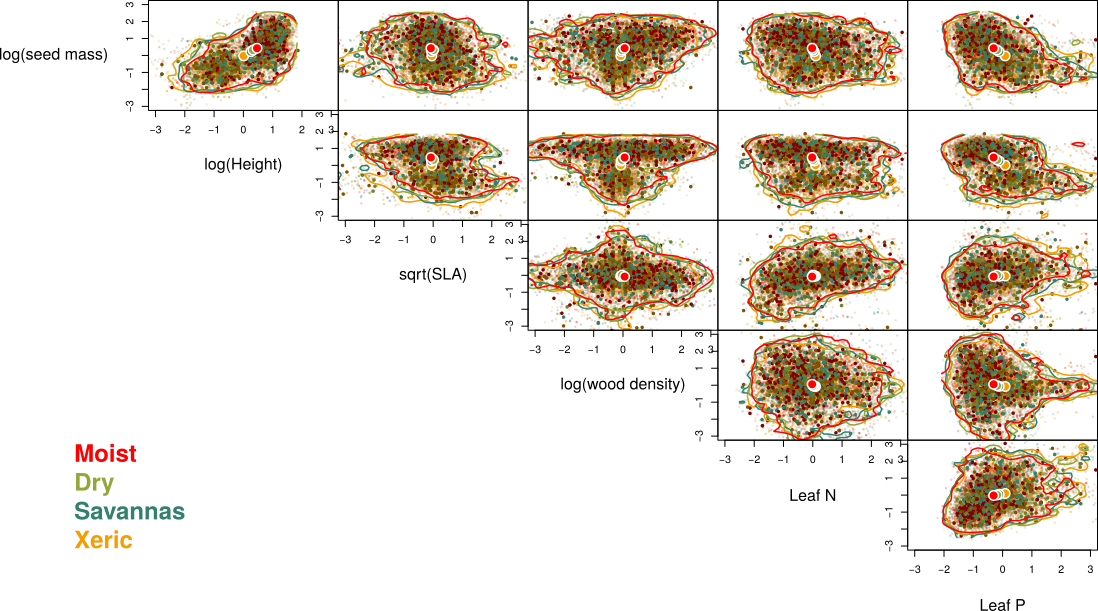
\includegraphics[width=0.245\textwidth]{./figures/Total_Moist_Dry_Savanna_Xeric.pdf}
	~
	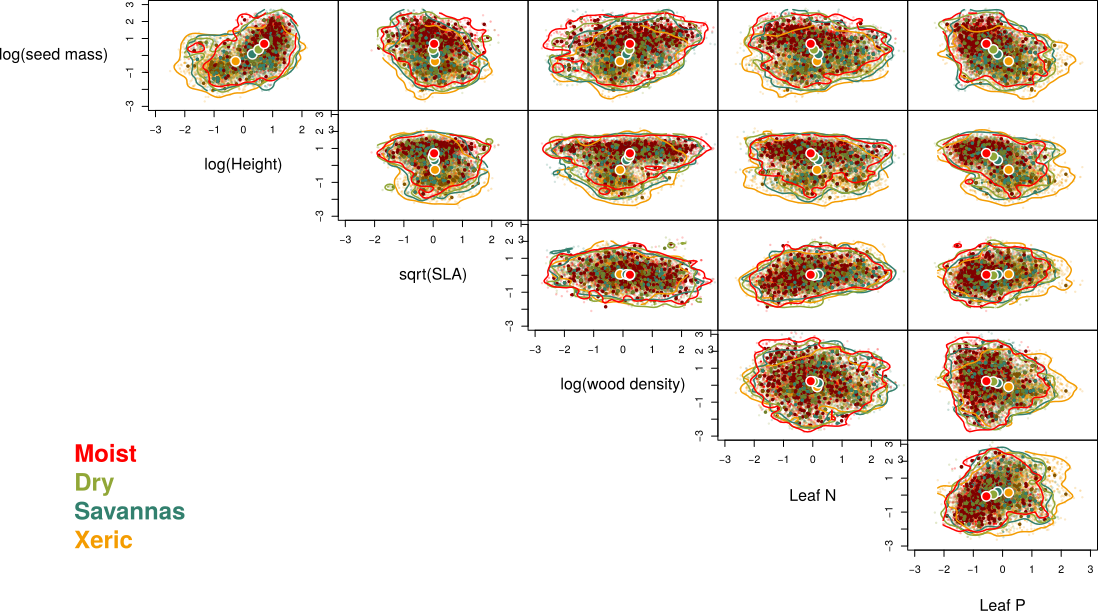
\includegraphics[width=0.245\textwidth]{./figures/Redun_Moist_Dry_Savanna_Xeric.pdf}
	\caption{Trait hypervolumes for tropical biomes using (A) the whole pool of species, and (B) using species that are functionally
redundant and widespread in each biome. Hypervolumes are shown in a 2D projection using the combination of all six trait axes implemented
in this study.}
	\label{fig:hypervolumes}
\end{figure}

Pairwise comparisons of species composition among biomes reveal three main clusters representing the tropical, temperate and polar climatic zones (Fig. \ref{fig:heatmaps}A), in agreement with the vast number of shared species within these regions as shown in Fig. \ref{fig:map}A. Pairwise comparisons of trait hypervolumes among biomes show a less clear clustering of climatic zones (Fig. \ref{fig:heatmaps}B). The pairwise comparison of trait hypervolumes among biomes using only those species considered as functionally redundant and widespread shows less overlap in trait spaces among and within climatic zones (Fig. \ref{fig:heatmaps}B). However, even though xeric woodlands are now clustered with the rest of tropical biomes, these habitats along with tropical grassland exhibit great overlap in functional space with temperate biomes such as Mediterranean woodlands and temperate grasslands. 

\end{multicols}
\end{block}



			\begin{alertblock}{Discussion}
			
The fact that common, widespread species are functionally redundant reinforces the notion that land plants across a wide range of environmental conditions share common characteristics near the core of the functional trait spectrum (Diaz et al., 2016; Wright et al., 2004). 

Despite extensive taxonomic and functional overlap among biomes, they do cluster into distinguishable, biogeographically and climatically sensible units, especially when the functional clustering is based on the most widespread and functionally common species in each biome. However, understanding the similarity in trait space among regions with similar environmental conditions is not sufficient to make accurate predictions of ecosystem function (Forrestel et al., 2017). Advancing these methods will require the not just a better characterization of trait variation within and between vegetation types, but also information on the biogeographic and phylogenetic history of species assemblages and the relative abundance of species within biomes.

      		\end{alertblock}

 \end{column}



  \begin{column}{\sepwid}\end{column}			% empty spacer column
  \begin{column}{\onecolwid}



	\begin{figure}[h]
		\centering
		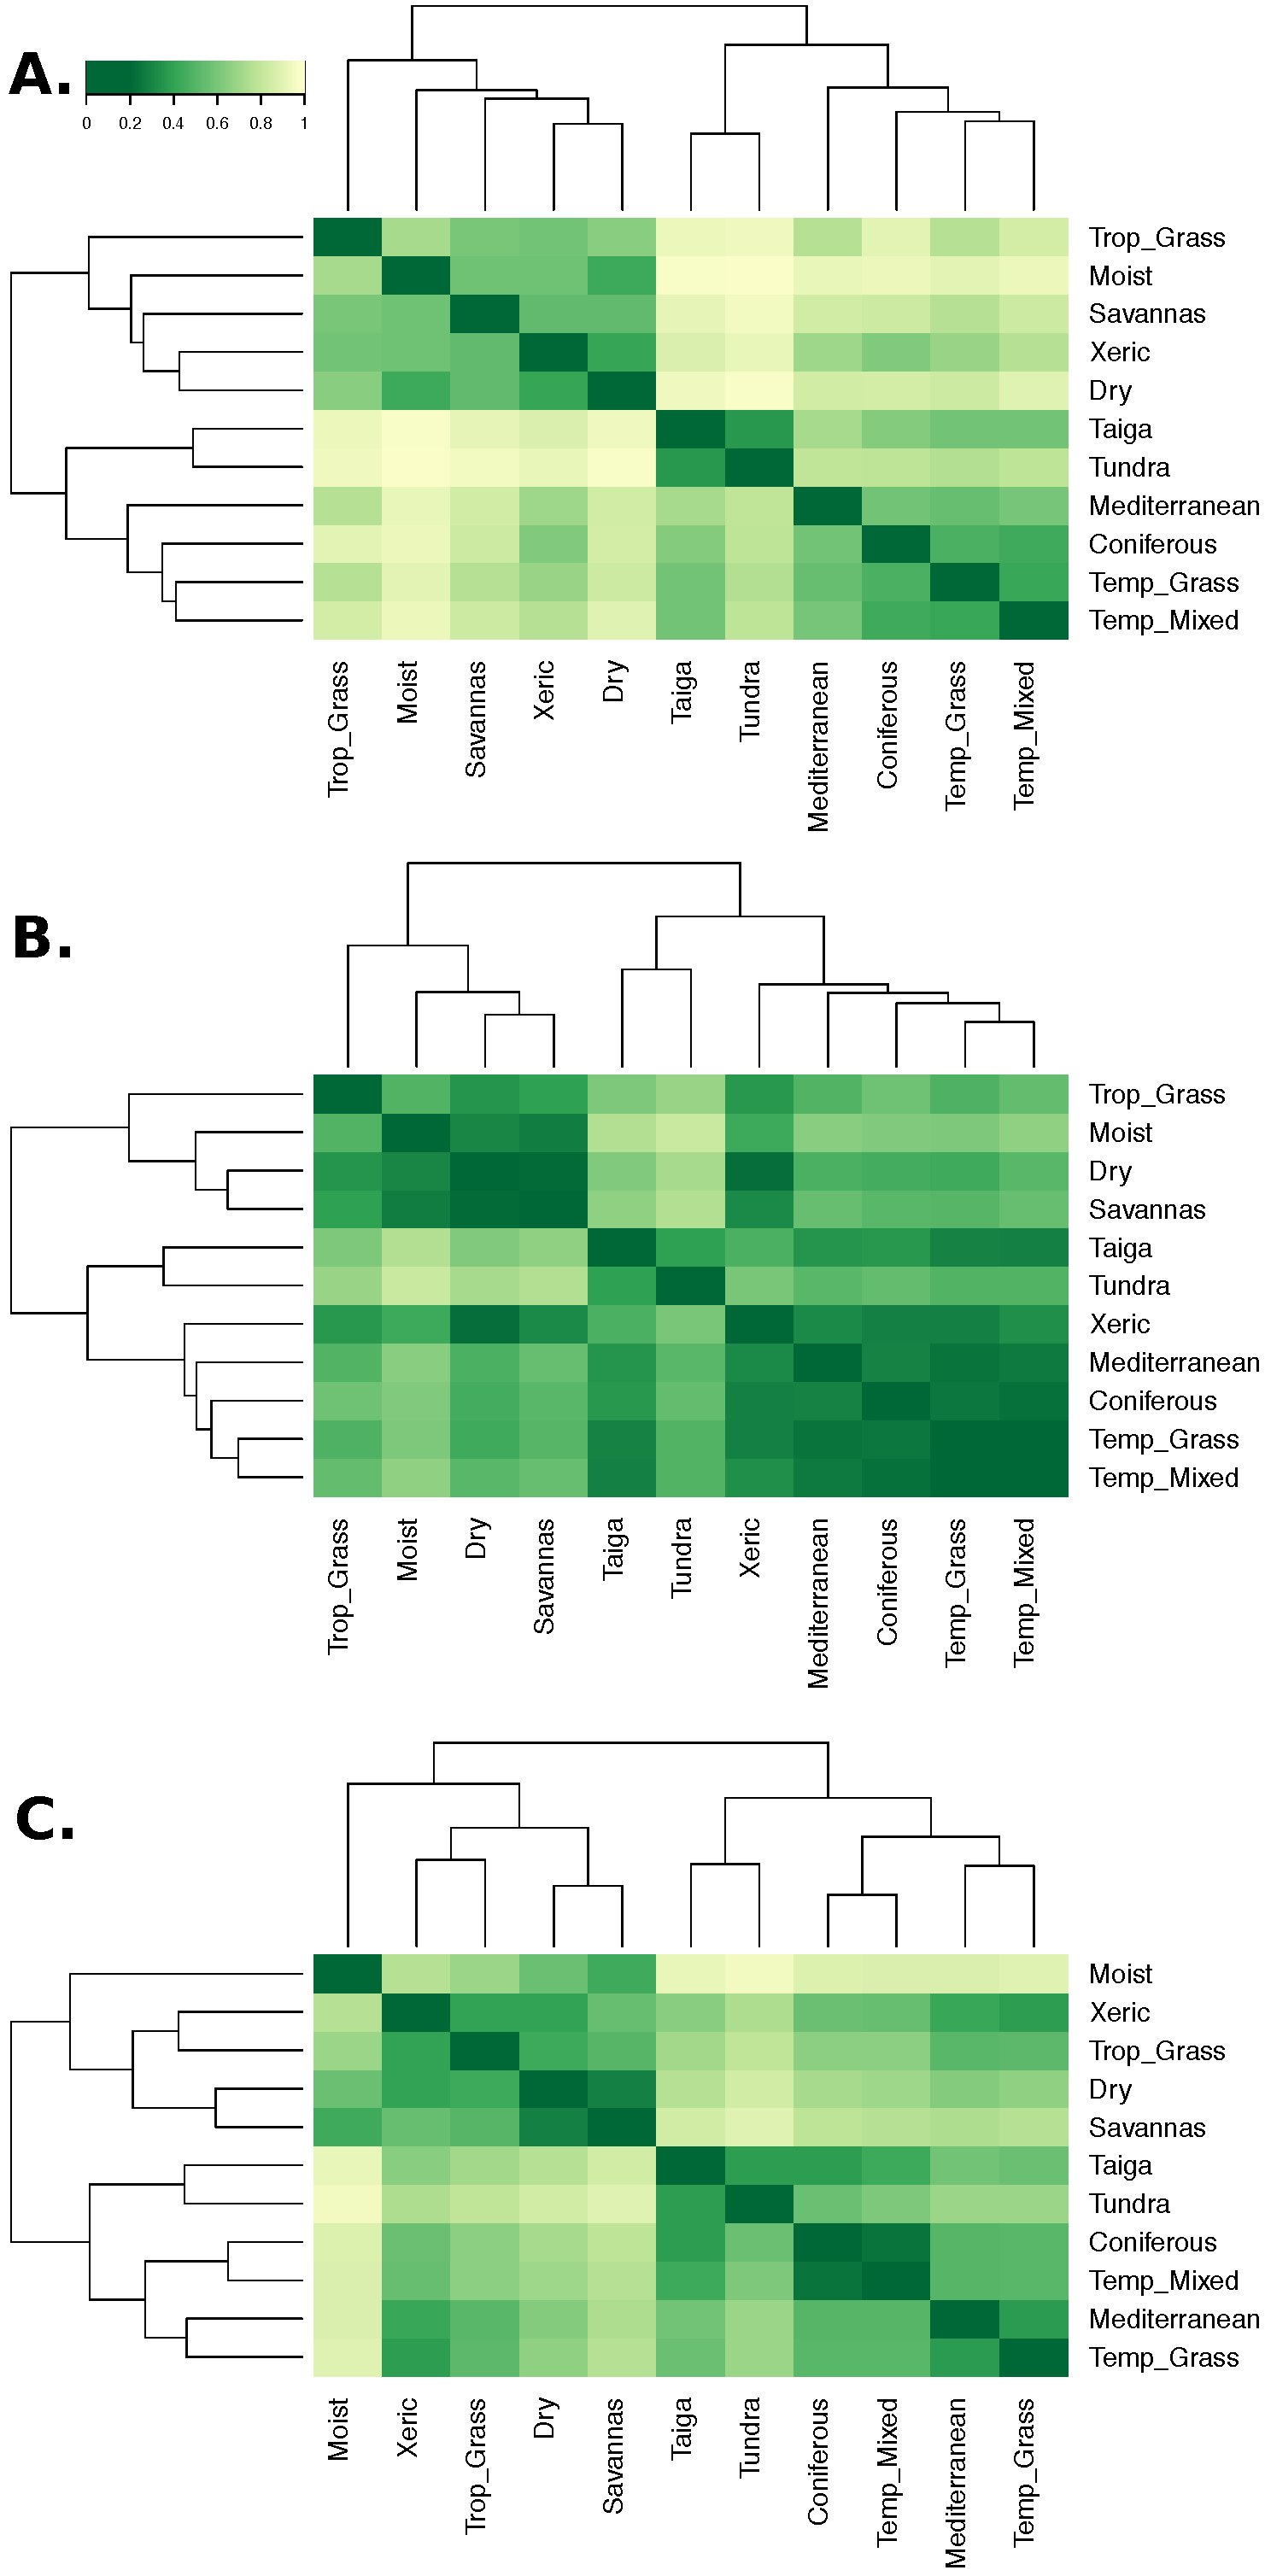
\includegraphics[width=0.6\textwidth]{./figures/heatmaps.pdf}
		\caption{(A) Pairwise dissimilarity in species composition among biomes. (B) Pairwise dissimilarity in trait hypervolumes (1-S\o rensen similarity) among biomes using the total number of species. (C) Pairwise dissimilarity in trait hypervolumes (1-S\o rensen similarity) among biomes using only those species that are considered as functionally redundant and widespread. The lighter the cell the greater the dissimilarity.}
		\label{fig:heatmaps}
	\end{figure}


      		\begin{alertblock}{Conclusions}
      		\begin{itemize}
      		\item Despite progress in the compilation and synthesis of primary biodiversity data, significant knowledge shortfalls persist that may limit our ability to quantify the functional biodiversity of biomes on continental to global scales.
      		
      		\item when only the widespread and functionally redundant species are considered, biomes can be more readily distinguished functionally, and patterns of dissimilarity between biomes appear to reflect a correspondence between climate and plant functional niche space.
      		\item Our results suggest that while the study of the functional diversity of biomes is still in its formative stages, further development of the field will yield insights linking evolution, biogeography, community assembly, and ecosystem function.
      		\end{itemize}

      		\end{alertblock}



    \vskip2ex

\begin{block}{References}

\scriptsize

	\begin{itemize}

	\item Blonder, B., Lamanna, C., Violle, C., and Enquist, B. J. Glob. Ecol. Biogeogr. \textbf{23}, 595-609 (2014).

	\item Blonder, B., Morrow, C. B., Maitner, B., Harris, D. J., Lamanna, C., Violle, C., et al. Methods Ecol. Evol. \textbf{9}, 305-319 (2018). 
	
	\item Diaz, S., Kattge, J., Cornelissen, J. H. C., Wright, I. J., Lavorel, S., Dray, S., et al. Nature \textbf{529}, 167 (2016).

	\item Enquist, B. J., Condit, R., Peet, R. K., Schildhauer, M., and Thiers, B. M. PeerJ Preprints No. e2615v1 (2016).
	
	\item Forrestel, E. J., Donoghue, M. J., Edwards, E. J., Jetz, W., du Toit, J. C. O., and Smith, M. D. Proc Natl Acad Sci \textbf{114}, 705–710 (2017). 

	\item Goldsmith, G. R., Morueta-Holme, N., Sandel, B., Fitz, E. D., Fitz, S. D., Boyle, B., et al. Methods Ecol. Evol. \textbf{7}, 960-965 (2016). 

	\item Goolsby, E. W., Bruggeman, J., and An\'e, C. Methods Ecol. Evol. \textbf{8}, 22-27 (2017).

	\item Smith, S. A., and Brown, J. W. Am. J. Bot. \textbf{105}, 302-314 (2018). 
	
	\item Wright, I. J., Reich, P. B., Westoby, M., Ackerly, D. D., Baruch, Z., Bongers, F., et al. Nature \textbf{428}, 821 (2004). 
		        
	\end{itemize}

\vspace{0.75in}

\end{block}


      		\begin{block}{Acknowledgments}
\scriptsize This study was conducted as a part of the BIEN Working Group (Principal Investigators: Brian J. Enquist, Brad Boyle, Richard Condit, Steven Dolins, Robert K. Peet, and Barbara M. Thiers) supported by the National Centre for Ecological Analysis and Synthesis, a center funded by the National Science Foundation (NSF Grant EF-0553768), the Univ. of California, Santa Barbara, and the State of California. The BIEN Working Group was also supported by the iPlant Collaborative (NSF Grant DBI- 0735191). We thank all the contributors for the invaluable data provided to the BIEN (http://bien.nceas.ucsb.edu/bien/people/data-contributors/).
      		\end{block}


    \vskip2ex

  \end{column}


  \begin{column}{\sepwid}\end{column}			% empty spacer column
 \end{columns}
\end{frame}
\end{document}
